\section{Introduction}

We consider an image sequence $f_{k}(x, y), k \in[1, K], x \in[1, M], y \in[1, N]$. In our case, in regard to a reference image, each following image in the sequence can be registered on the reference by a rotation of angle $\theta_k$ and a translation by a vector $\tau_k = (x-x_k, y-y_k)$. In our situation, we know there is no rotation in the sequence so we want to estimate the parameters $\tau_k$ for each image.


\begin{align*}
\forall \; k>1, \quad f_k(x, y) &= f_{1}\left(x-x_{k}, y-y_{k}\right) + b(x, y) \\
\forall \; k>1, \quad f_{k}(x_i, y_j) &= f_{1}\left(x_i-x_{k}, y_j-y_{k}\right) + b_{k}(x_i, y_j)
\end{align*}

Here, $f$ is probabilist due to the nature of $b$, while $f_1$ is determinist. We sample the signal so it is now a serie of discret value, taken at pixel position $(i, j)$.

In the case of a normalized signal, because the log-likelyhood shows a mean-square difference, one can show that its derivative is proportional to the scalar product of the observed signal $f_k$ and the model signal $f_1$. If the noise is gaussian, then MLE is optimal, and thus the matched filter is optimal. If the noise is correlated (covariance matrix $\Gamma$), one can substitute the signal to whitened the noise : consider $\Gamma^{-1} . f$ and $\Gamma^{-1} . r(x, y)$.

The estimator is then :


\begin{equation}
\hat{\tau_k} = arg \; max \left[ f_k^T\Gamma^{-1} f_1 \right]
\end{equation}

And if the noise is uncorrelated, then $\Gamma^{-1} = Id$.

\section{Registration algorithm}
We consider a white noise, and we want to express the scalar product :


\begin{equation}
f_k^T \cdot f_1 = \sum_{x,y} f_k . f_1 = a . A(\tau_k,\tau_1) + b'(\tau_k), \quad b'(\tau_k) = b^T f_1(\tau_k)
\end{equation}

We suppose that the ambiguity function $A$ is symetrical with respect to $\theta_0$ and thus is unbiased.

The ambiguity function is equal to the autocorrelation function of the reference signal $f_1$ with $\tau$ the translation and $\tau_k$ the true translation for image $k$ : $ A(\tau, \tau_k) = C(\tau, \tau_k) $. 

By computing the autocorrelation in the Fourier domain, we can estimate the translation of the centers of the two images. To test the obtain translation vector, one could simply roll the unregistered image according to that vector and then substract the two images and observe a uniform noise. If some shapes are still visible then the shift was not right.

\subsection{Results}
Here the image is of shape (300 x 500) thus the center is located at (150,250). We select the second image of the sequence and computes the correlation between the reference image and the selected image to find a translation vector (1,4).

\begin{figure}[h]
	\centering
	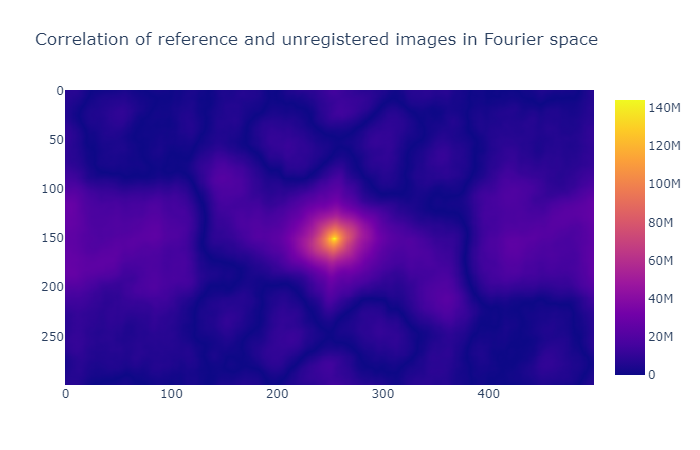
\includegraphics[scale=0.5]{corr-1.png}
	\caption{Correlation between reference image and second unregistered image}
	\label{fig:corr-1}
\end{figure}

We then roll the selected image according to that translation vector and substract the two : we observe a white noise over the screen so we conclude that the estimated translation was correct.

\begin{figure}[h]
    \centering
    \subfloat[Substraction before rolling]{
        \centering
        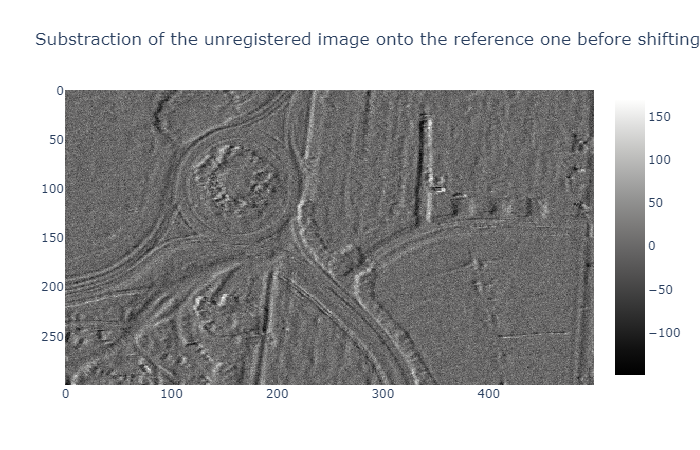
\includegraphics[width=0.45\textwidth]{substract-1.png}
        \label{fig:substract-before}
    }
	\subfloat[Substraction after rolling]{
		\centering
        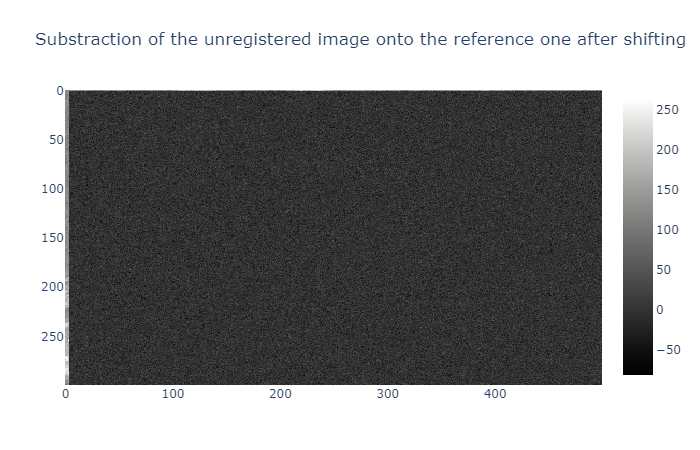
\includegraphics[width=0.45\textwidth]{substract-2.png}
        \label{fig:substract-after}
    }
	\caption{Registration check}
\end{figure}

Because the defined algorithm has been verified, we present here the translation vector (in red) onto the reference image.

\begin{figure}[h]
    \centering
    \subfloat[Necessary translation for registering the image]{
        \centering
        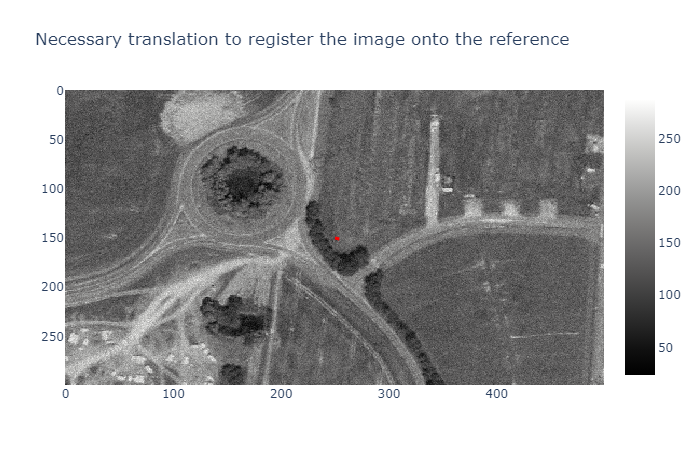
\includegraphics[width=0.45\textwidth]{shift.png}
        \label{fig:translation}
    }
	\subfloat[zoom onto the translation vector]{
		\centering
        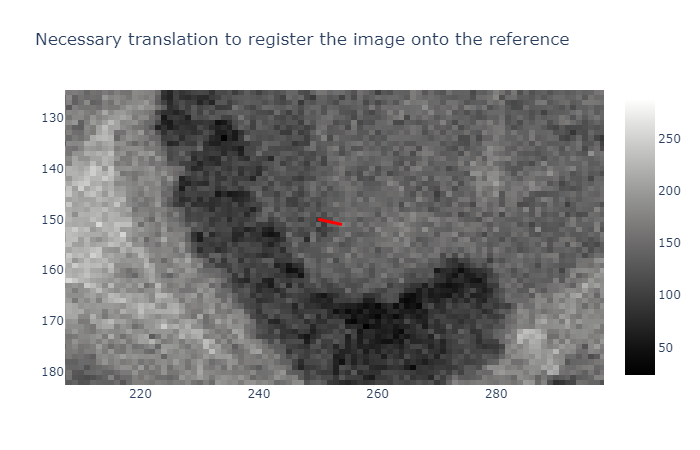
\includegraphics[width=0.45\textwidth]{shift-detail.png}
        \label{fig:translation-detail}
    }
	\caption{Translation vector}
\end{figure}

\pagebreak
\subsection{Blocks}
For sake of memory resources or because of time calculation, it is not always possible do compute the Fourier transform of the whole image. In this case, one has to compute the shift from a small region of the reference image. We will take a $30 \times 30$ pixels wide region.

The goal is then to choose the region of the image that leads to the highest precision for shift estimation.

Here we present 5 blocks that we chose according to be different parts of the image. We also plot the Harris corner detection at 1\% of the maximum of the Harris score.

\begin{figure}[h]
	\centering
	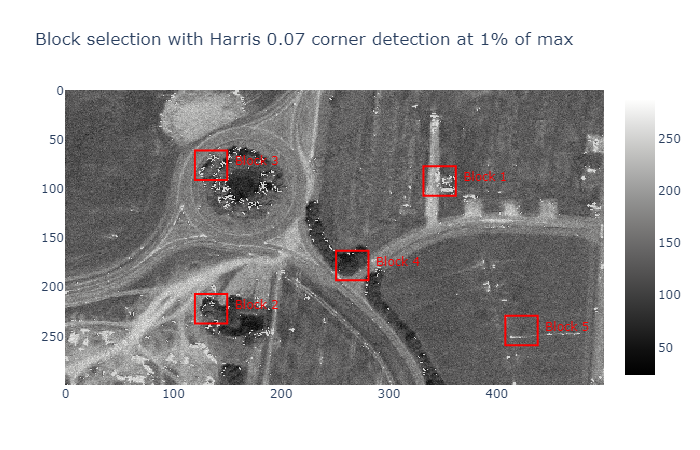
\includegraphics[scale=0.5]{blocks.png}
	\caption{Blocks on the reference image}
	\label{fig:blocks}
\end{figure}

We then need to find the different position of the block onto the reference and the unregistered image. For that, we compute the correlation between the block and the reference image, which leads to the position of the block on the reference, and we compute the correlation of the block and the unregistered image, which gives the corresponding position on the unregistered image. By computing the difference one should find the neccessary shift to register the image. 

\begin{figure}[h]
    \centering
    \subfloat[correlation over the reference image]{
        \centering
        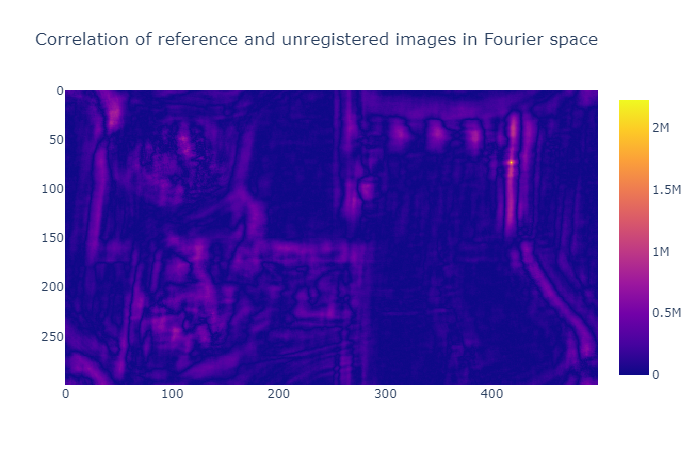
\includegraphics[width=0.45\textwidth]{block-ref.png}
        \label{fig:corr-ref}
    }
	\subfloat[correlation over the unregistered image]{
		\centering
        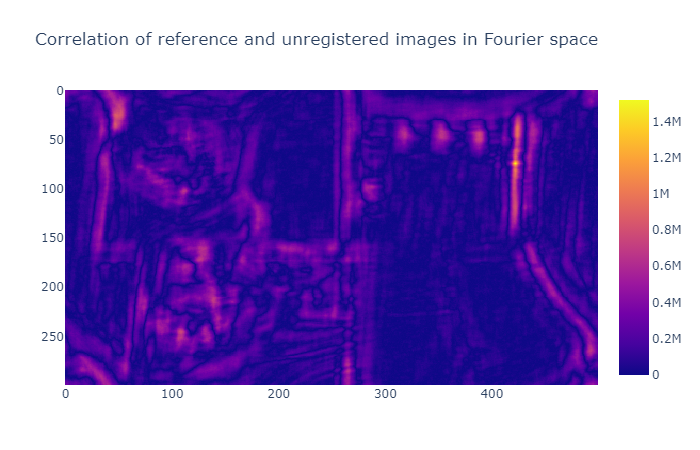
\includegraphics[width=0.45\textwidth]{block-unregistered.png}
        \label{fig:corr-unregistered}
    }
	\caption{Correlation over 30 x 30 pixels blocks}
\end{figure}


We then compare the translation vectors with the true one, checked with the substraction test.
\begin{figure}[h]
	\centering
	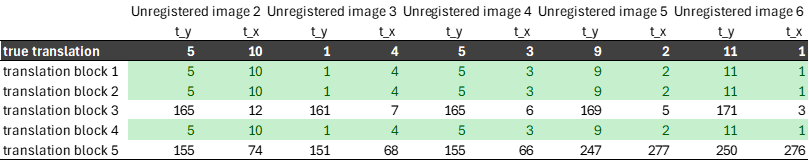
\includegraphics[scale=0.65]{blocks-data.png}
	\caption{Computed translation vector}
	\label{fig:blocks-data}
\end{figure}

We observe that the blocks 1, 2 and 4 always give the correct translation vector. This is also the blocks the most filled with Harris corners, which are points with a maximum gradient in intensity. We thus suggest that to find the optimal block, one should focus on a block with high intensity variations.

\subsection{Optimality}
To find the optimal block for shift estimation, one can compute the Fisher information matrix (see the course p.66) and finally get the CRLB for $x_k, y_k$ :


\begin{align*}
VAR(\hat{x_k}) & = \frac{SNR^{-1}}{4\pi^2} . \frac{\overline{\Delta \nu \nu^2}}{\overline{\Delta \mu \mu^2} \times \overline{\Delta \nu \nu^2} - \left( \overline{\Delta \mu \nu^2} \right)^2} \\
VAR(\hat{y_k}) & = \frac{SNR^{-1}}{4\pi^2} . \frac{\overline{\Delta \mu \mu^2}}{\overline{\Delta \mu \mu^2} \times \overline{\Delta \nu \nu^2} - \left( \overline{\Delta \mu \nu^2} \right)^2}
\end{align*}


Where $\mu$ is the fourier variable for $x$ and $\nu$ is the fourier variable for $y$, and $\sqrt{\overline{\Delta \mu^2}}$ represents the spectral "width" of the signal along the x-axis. We have :

$$
\sqrt{\overline{\Delta \mu^2}} = \iint \nu^2 |\hat{f}(\mu,\nu)|^2 d\nu d\mu
$$

Here, because the noisy signal is separable, we have $ \overline{\Delta \mu \nu^2} = 0 $. The we get :


\begin{align*}
VAR(\hat{x_k}) & = \frac{SNR^{-1}}{4\pi^2\overline{\Delta \mu \mu^2}} \\
VAR(\hat{y_k}) & = \frac{SNR^{-1}}{4\pi^2\overline{\Delta \nu \nu^2}}
\end{align*}

\section{Detection using the matched filter}
In radar detection, one must test two hypotheses :
\begin{itemize}
    \item Hypothesis H0 $\quad x(t)=b(t)$
    \item Hypothesis H1 $\quad x(t)=a s(t)+b(t)$
\end{itemize}
where :

\begin{itemize}
    \item $x(t)$ is the measured signal,
    \item $s(t)$ is the emitted pulse, known by the user,
    \item $a$ is the attenuation factor,
    \item $b(t)$ is the noise on the measure.
\end{itemize}


We assume that we know where the target may be. We only want to know if the target is or not at this position. We first only consider the detection problem. In reality, we don't know if there is a target, neither its possible position. We must detect and estimate at the same time. That is what we will study in the image processing application.

If the noise $b(t)$ is white, the optimal detector (matched filter) is a correlation between the measured signal and the emitted pulse :

$$
F(\theta)=\int x(t) s(t-\theta) d t
$$

We only need to calculate this expression at one point (chosen here as 0 ) if we assume that the position is known. Thus, we have to test :

$$
F(0)=\int x(t) s(t) d t
$$

This value is then compared to a threshold in order to take a decision.

\pagebreak
\subsection{Noisy gaussian pulse}
The SNR (Signal to Noise Ratio) of the detection is defined by :

$$
\mathrm{SNR}=\frac{a^{2} E_{s}}{\sigma^{2}} \quad \mathrm{SNR}_{\mathrm{dB}}=10 \log \left(\frac{a^{2} E_{s}}{\sigma^{2}}\right)
$$

where $E_{s}$ is the energy of the emitted pulse: $E_{s}=\int|s(t)|^{2} d t$ and $\sigma^{2}$ the variance of the noise $b(t)$. We assume that the temporal shape of the pulse is gaussian and the attenuation factor $a=1$. We suppose also that $b(t)$ is a gaussian white noise.

\begin{figure}[h]
	\centering
	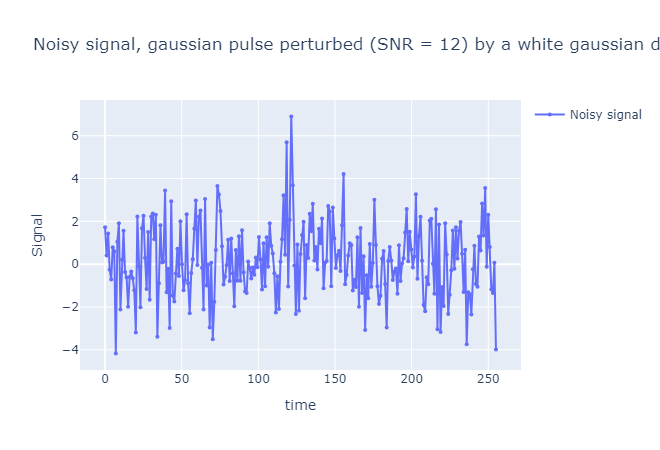
\includegraphics[scale=0.55]{noisy.png}
	\caption{Noisy signal}
	\label{fig:noisy}
\end{figure}

\begin{figure}[h]
    \centering
    \subfloat[Clean signal]{
        \centering
        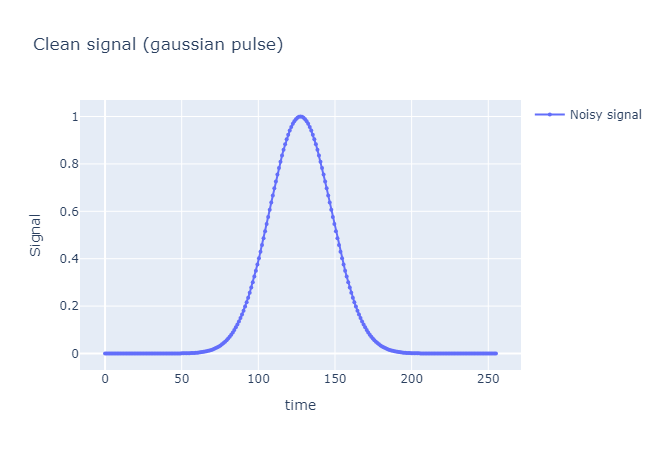
\includegraphics[width=0.45\textwidth]{clean-signal.png}
        \label{fig:clean}
    }
	\subfloat[Filtered signal]{
		\centering
        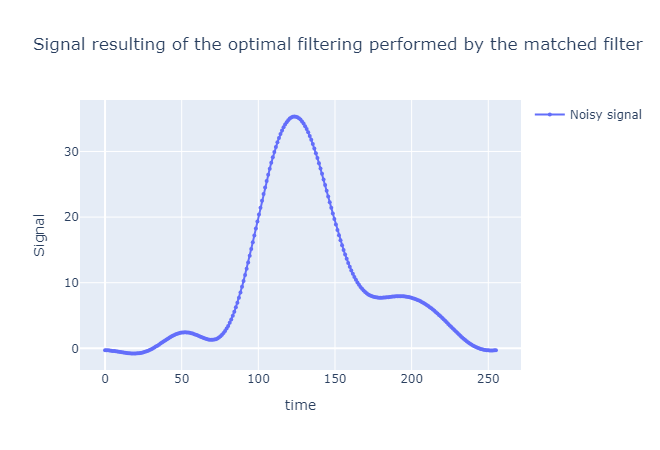
\includegraphics[width=0.45\textwidth]{filtered.png}
        \label{fig:filtered}
    }
	\caption{Clean and filtered signal}
\end{figure}

\begin{figure}[h]
	\centering
	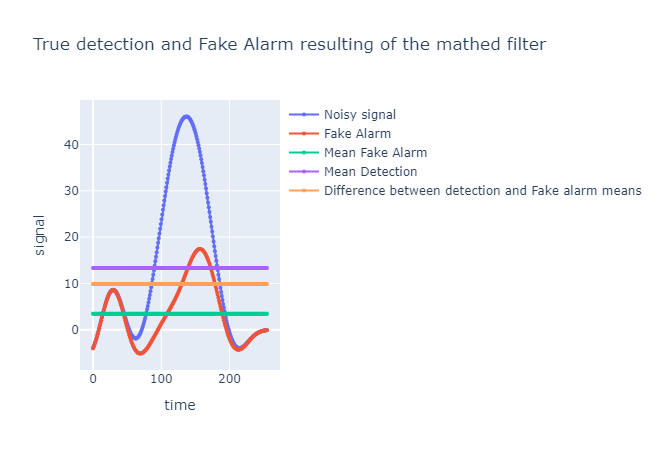
\includegraphics[scale=0.55]{fake-alarm.png}
	\caption{Fake alarm and detection}
	\label{fig:fake-detection}
\end{figure}

We run the script several times, and we observe that the mean of the Fake Alarm signal seem always inferior to the difference between the means of the FA signal and the Detection signal (which remain constant over iterations, approximately equals to 10). On the contrary, the mean of the Detection signal is sometimes superior, sometimes inferior to this threshold.

As a result, one can define the difference between the means as a threshold to compare the Fake Alarm mean to.

Over the iteration, one can also observe that the mean of the Detection signal seems always superior to the mean of the Fake Alarm signal. Thus, one could try to see if those means converge toward a certain value over the iterations in order to see if another threshold could be defined.

However, one could notice that here, the noisy signal is made of the clean signal without any translation over time. Thus, it is not needed to compute the whole correlation of the signal : one could simply look at the value of the correlation function at $\theta = 0 $ (i.e. no translation at all). In this case, it seems that 25 is a suitable threshold.

Notice that in the case of a translated clean signal, one could look at the maximum of the correlation function to estimate the value of the translation in the case of a detection.

\subsection{ROC curves}
The Receiver Operating Characteristic is a curve of the detection probability versus false alarm probability for all the threshold possible values. According to the following overlaying histograms, the optimal threshold is located at the intersection of the two histograms. The threshold defines what values are considered as a detection and which are not. Because the histograms overlay, the threshold implies that a portion of the considered detected values are not linked to an actual detection (fake alarm detection), this is illustrated by the part of the H0 hypothesis histogram above the defined threshold. It reciprocaly implies that a portion of the values corresponding to an actual detection are not considered as so (non-detection values, corresponding to the H1 hypothesis histogram values under the threshold).

\begin{figure}[h]
	\centering
	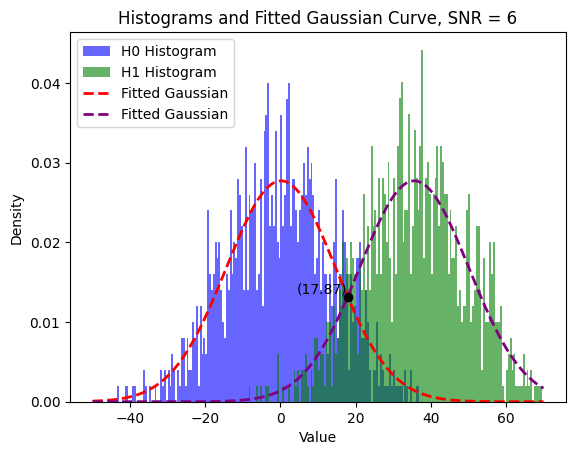
\includegraphics[scale=0.65]{hist_6.png}
	\caption{Histograms of H0 and H1 with SNR = 6}
	\label{fig:hist6}
\end{figure}

\begin{figure}[h]
    \centering
	\subfloat[Integration at optimal threshold]{
		\centering
        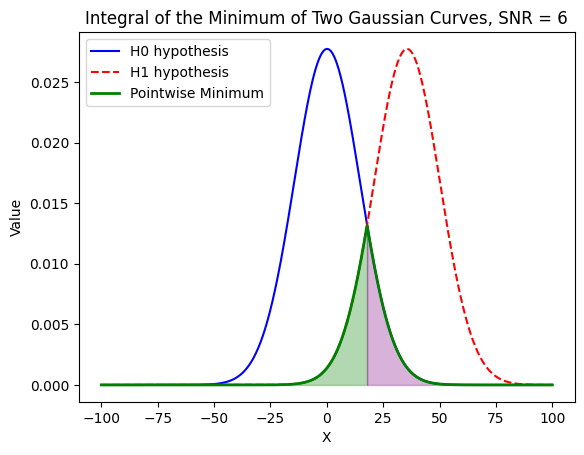
\includegraphics[width=0.45\textwidth]{hist_min_6.png}
        \label{fig:integ6}
    }
    \subfloat[ROC curve]{
		\centering
        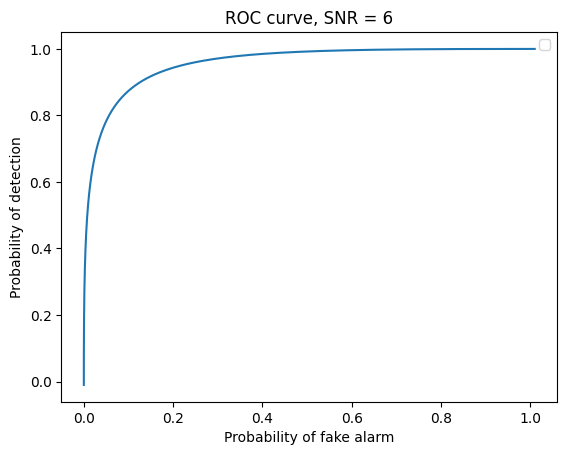
\includegraphics[width=0.45\textwidth]{ROC_6.png}
        \label{fig:ROC6}
    }
	\caption{H0 and H1 hypothesis for SNR = 6}
\end{figure}

On figure \ref{fig:hist6} one could see that the optimal threshold defined as 25 in the empirical tests above can be adjusted to 17.87, a value that is quite stable over iterations. However, it leads to a higher probability of detecting fake alarm than the empirical threshold.

So, one could plot the probability of fake alarm detection according to a varaition of the threshold, and one could also do the same for the non-detection case. Thoses probabilities are defined by the area under the histograms in the fake alarm and non-detection values, and thus thoses curves would be varying with the SNR. So to sum up, one could plot the ROC curve as a function of the SNR. To do that, we will need to fit the distribution of the two hypothesis with a gaussian curve in order to find the intersection point and computes the probabilities.

A ROC curve with an inflection point in the top-left corner (0, 1) represents an optimal detector. In this scenario, there are no false positives or false negatives. This behavior is typically observed in simulations when the SNR reaches values of 16 or 20.

\begin{figure}[h]
	\centering
	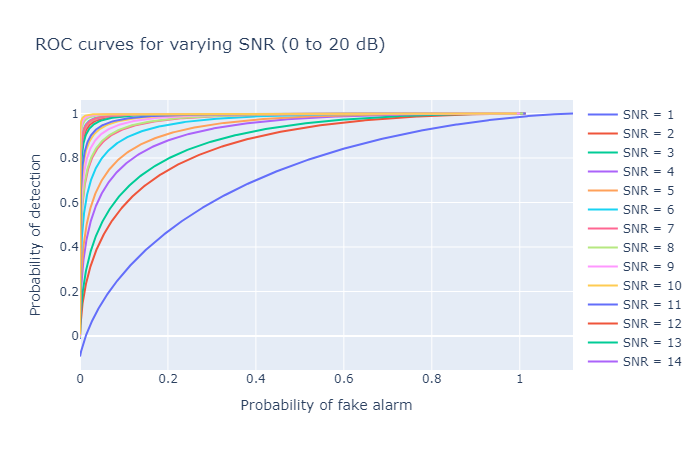
\includegraphics[scale=0.55]{ROCs.png}
	\caption{ROC curves for varying SNR}
	\label{fig:ROCs}
\end{figure}

As the signal-to-noise ratio (SNR) decreases, the target signal becomes harder to detect as it is increasingly masked by surrounding noise. Consequently, the system's ability to correctly detect the signal decreases, leading to more false positives (detection errors) and fewer true positives (correct detections). Graphically, as the SNR approaches zero, the inflection point of the ROC curve shifts closer to the diagonal from (0, 0) to (1, 1), representing a worst-case detector governed by chance.

This diagonal splits the ROC space: points above it indicate good detection results (better than chance), while points below it (which don't occur in practice) would represent worse-than-random results.





\subsection{OCR in a text}
Here we wish to detect a character in a text. In this case we don't know its position. We must address the "detection-estimation" problem. The matched filter can be used for that purpose :
\begin{itemize}
    \item a peak in the matched filter output indicate if the character is detected,
    \item the peak position gives an estimate of the character position.
\end{itemize}

First, we need to extract a perfect caracter from the perfect image in order to perform a correlation between the image and the selected caracter. Then, if the process is a success, we will perform the correlation between the same caracter and a noisy image to test the robustness of the matched filter.

In order to test both the detection and estimation performed by the match filter, we decide to draw a circle centered on each estimated position of detected correlation on the image.

\begin{figure}[h]
    \centering
    \subfloat[Correlation with character]{
        \centering
        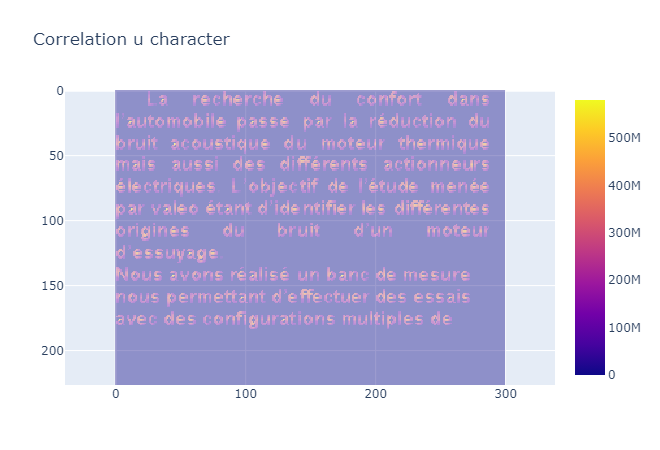
\includegraphics[width=0.45\textwidth]{correlation-text.png}
        \label{fig:detection-correlation}
    }
	\subfloat[Detected characters]{
		\centering
        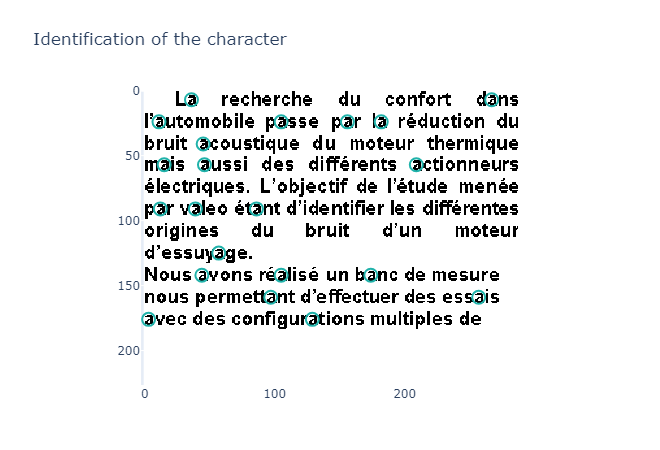
\includegraphics[width=0.45\textwidth]{correlation-text-shape.png}
        \label{fig:detection-shape}
    }
	\caption{Detection in perfect text}
\end{figure}

Here we present the detection of the letter "a" which was a success due to its unique features. This was not the case with the letter "u" nor "s" because their features ressemble too much to other letters and thus a lot of fake alarm occured. In the picture below, we present the detection in a noisy image, were the background and the letters are not uniform, we observe a gradient of intensity from the top to the bottom of the image, thus leading to a correlation value higher in the high intensity zones, and thus a lot of fake alarm. This illustrate the need of image pre-processing before trying use detection algorithm such as the matched filter.

\begin{figure}[h]
    \centering
    \subfloat[Intensity background gradient over image]{
        \centering
        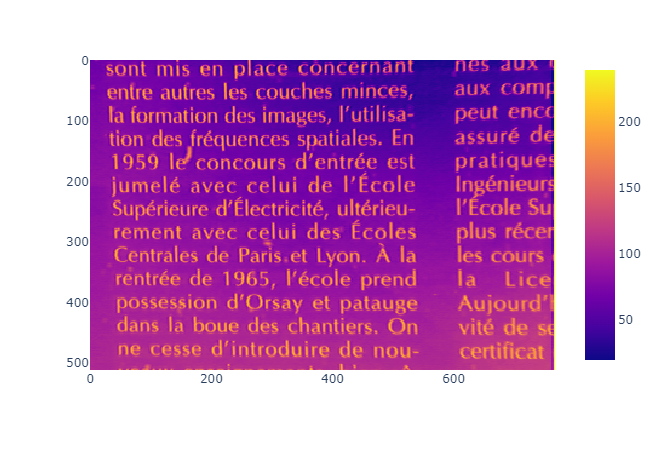
\includegraphics[width=0.45\textwidth]{noisy-text.png}
        \label{fig:}
    }
	\subfloat[fake-alarm]{
		\centering
        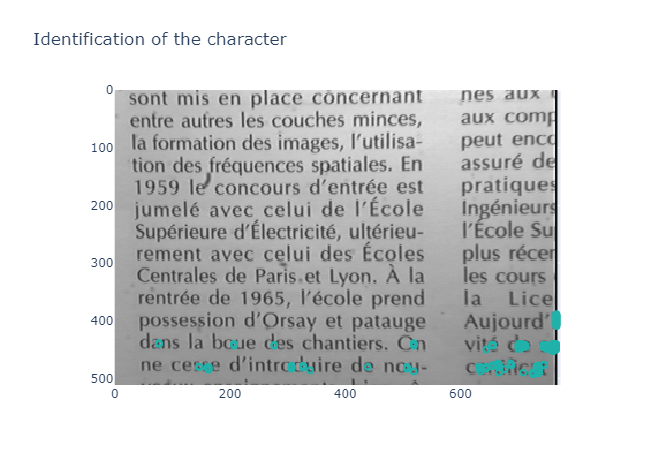
\includegraphics[width=0.45\textwidth]{noisy-text-shape.png}
        \label{fig:fake-alarm}
    }
	\caption{Fake alarm on noisy text}
\end{figure}
\pagebreak

\section{Conclusion}

The results of this study highlight the relevance of using a matched filter for both estimation and detection tasks. For estimating inter-frame displacements, the filter proved to be highly effective. However, in detection contexts, its performance strongly depends on situation-specific parameters. In particular, the signal-to-noise ratio (SNR) significantly impacts the likelihood of false alarms and, therefore, the overall detection efficiency.